\documentclass[a4paper,12pt]{article}
\usepackage{amsmath,amssymb,amsfonts,amsthm}
\usepackage{tikz}
\usepackage [utf8x] {inputenc}
\usepackage [T2A] {fontenc} 
\usepackage[russian]{babel}
\usepackage{cmap} 
\usepackage{ gensymb }
% Так ссылки в PDF будут активны
\usepackage[unicode]{hyperref}
\usepackage{ textcomp }
\usepackage{indentfirst}
\usepackage[version=3]{mhchem}
\usepackage{wrapfig}
% вы сможете вставлять картинки командой \includegraphics[width=0.7\textwidth]{ИМЯ ФАЙЛА}
% получается подключать, как минимум, файлы .pdf, .jpg, .png.
\usepackage{graphicx}
% Если вы хотите явно указать поля:
\usepackage[margin=1in]{geometry}
% Или если вы хотите задать поля менее явно (чем больше DIV, тем больше места под текст):
% \usepackage[DIV=10]{typearea}
\usepackage{fancyhdr}
\pagestyle{fancy}
\makeatletter % сделать "@" "буквой", а не "спецсимволом" - можно использовать "служебные" команды, содержащие @ в названии
\fancyhead[L]{\footnotesize Оптика}%Это будет написано вверху страницы слева
\fancyhead[R]{\footnotesize ФФКЭ МФТИ}
\fancyfoot[R]{\thepage}%номер страницы —- внизу справа
\fancyfoot[C]{}%по центру внизу страницы пусто

\renewcommand{\maketitle}{%
	\noindent{\bfseries\scshape\large\@title\ \mdseries\upshape}\par
	\noindent {\large\itshape\@author}
	\vskip 2ex}
\makeatother
\def\dd#1#2{\frac{\partial#1}{\partial#2}}


\title{4.7.3 \\ Поляризация}
\author{Богатова Екатерина} 
\date{3 апреля 2022 г.}

\begin{document}
\maketitle
\textbf{Цель работы:}
ознакомление с методами получения и анализа поляризованного света.

\textbf{В работе используются:}
оптическая скамья с осветителем; зелёный светофильтр; два поляроида; чёрное зеркало; полированная эбонитовая пластинка; стопа стеклянных пластинок; слюдяные пластинки разной толщины; пластинки в 1/4 и 1/2 длины волны; пластинка в одну длину волны для зелёного света (пластинка чувствительного оттенка).

\section{Теория}
\begin{wrapfigure}{r}{0.35\linewidth} 
	\includegraphics[width=\linewidth]{1}
	\caption{Разложение элептической поляризации на линейные компоненты}
	\label{ris 1}
\end{wrapfigure}
При помощи специальных приспособлений (поляризаторов), естественный свет может быть поляризован. Наиболее общим типом поляризации является \textit{эллиптическая поляризация}. В эллиптически поляризованной световой волне конец вектора \textbf{E} в данной точке пространства описывает некоторый эллипс. Линейно поляризованный свет можно рассматривать как частный случай эллиптически поляризованного света, когда эллипс поляризации вырождается в отрезок прямой линии; другим частным случаем является круговая
поляризация (эллипс поляризации является окружностью). \par
Для получения линейно поляризованного света применяются специальные оптические приспособления — поляризаторы. Направление колебаний электрического вектора в волне, прошедшей через поляризатор, называется
разрешенным направлением поляризатора. Всякий поляризатор может быть использован для исследования поляризованного света, т. е. в качестве анализатора. Интенсивность I линейно поляризованного света после прохождения через анализатор зависит от угла, образованного плоскостью колебаний с разрешенным направлением анализатора:
\begin{equation}
    I = I_0 \cos 2\alpha.  
\end{equation}
Соотношение (1) носит название \textit{закона Малюса}. \par
Отраженный от диэлектрика свет всегда частично поляризован. Степень поляризации света, отраженного от диэлектрической пластинки в воздух, зависит от показателя преломления диэлектрика $n$ и от угла падения $\varphi$. Как следует из формул Френеля, полная поляризация отраженного света достигается
при падении под \textit{углом Брюстера}, который определяется соотношением
\begin{equation}
    \tg \varphi = n.   
\end{equation}

В этом случае плоскость колебаний электрического вектора в отраженном свете перпендикулярна плоскости падения. Для увеличения степени поляризации преломлённого света используют стопу стеклянных пластинок, расположенных под углом Брюстера к падающему свету. \par

\textbf{Определение направления разрешенной плоскости колебаний поляроида.}\par
Луч света, прошедший поляроид и отразившийся от чёрного зеркала, имеет минимальную интенсивность при выполнении двух условий: во-первых, свет падает на отражающую поверхность под углом Брюстера, и во-вторых, в падающем пучке вектор E лежит в плоскости падения. \par
Вращая поляроид вокруг направления луча и чёрное зеркало вокруг оси, перпендикулярной лучу, методом последовательных приближений можно добиться минимальной яркости луча, отражённого от зеркала, и таким образом определить разрешённое направление поляроида. По углу поворота зеркала можно определить коэффициент преломления материала, из которого изготовлено зеркало \par

\textbf{Получение элептически поляризованного света и его анализ.}\par
Эллиптически поляризованный свет можно получить из линейно поляризованного с
помощью двоякопреломляющих кристаллических пластинок.

Двоякопреломляющая пластинка имеет два взаимно перпендикулярных главных направления, совпадающих с осями эллипсоида диэлектрической проницаемости. Волны, поляризованные вдоль главных направлений, распространяются в пластинке с разными скоростями, не изменяя характера своей поляризации. Обозначим показатели преломления для главных волн через $ n_x $ и $ n_y $, где $ x $ и $ y $ --- главные направления кристаллической пластинки. На входе пластинки $ E_x $ и $ E_y $ находятся в фазе, однако на выходе из-за разности скоростей между ними появляется разность хода $ d(n_x - n_y) $, при этом сдвиг фаз определяется соотношением:
\begin{equation}\label{}
    \Delta \phi =  \dfrac{2\pi}{m} = k d(n_x - n_y)
\end{equation}

Анализ эллиптически поляризованного света сводится к нахождению главных осей
эллипса поляризации и к определению направления вращения электрического вектора.

Главные оси эллипса поляризации определяются с помощью анализатора по максимуму и минимуму интенсивности проходящего света. Направление вращения электрического вектора может быть найдено с помощью пластинки в четверть длины волны, для которой известно, какая из главных волн, $ E_x $ или $ E_y $, имеет б\'{o}льшую скорость распространения.

\textbf{Пластинка чувствительного оттенка}\par
\begin{wrapfigure}{l}{0.35\linewidth}
	\includegraphics[width=\linewidth]{3}
	\caption{Пластинка чувствительного оттенка}
	\label{ris 3}
\end{wrapfigure}

Установить какому из двух главных направлений пластинки $\lambda/4$ соответствует большая скорость распространения света можно различными способами, например с помощью пластинки чувствительного оттенка.

Пластинка имеет форму стрелы (рис. 2), вдоль оси которой расположено главное направление, соответствующее большей скорости распространения.

Если пластинка чувствительного оттенка помещена между скрещенными поляроидами и главные направления пластинки не параллельны направлениям разрешённых колебаний поляроидов, то при освещении белым светом пластинка кажется окрашенной в лилово-красный цвет.

Если между скрещенными поляроидами поместить пластинку чувствительного оттенка и пластинку в $ \lambda/4 $ так, чтобы их главные
направления совпадали, то проходящий свет будет казаться зеленовато-голубым.
Если же главные направления, соответствующие большей скорости распространения, у пластинки чувствительного оттенка и у пластинки
в $ \lambda/4 $ окажутся перпендикулярными, то проходящий свет приобретёт
оранжево-желтую окраску.

Изменение цвета позволяет, таким образом, определить, какое из
главных направлений пластинки в $ \lambda/4 $ соответствует большей скорости
распространения.

\textbf{Интерференция поляризованных лучей.}\par
\begin{wrapfigure}{r}{0.35\linewidth}
	\includegraphics[width=\linewidth]{4}
	\caption{К объяснению интерференции поляризованных лучей}
	\label{ris 4}
\end{wrapfigure}

Тонкие двоякопреломляющие пластинки, помещённые между поляроидами, кажутся окрашенными. Эта окраска может быть истолкована как результат интерференции поляризованных лучей. На рис. 3 представлена схема для
случая скрещенных поляроидов.

Здесь $ p1p'1 $ --- разрешённое направление колебаний поляризатора
(первого поляроида); $ x, y $ --- координатная система, связанная с главны-
ми направлениями двоякопреломляющей пластинки; $ p2p'2 $ --- разрешённое направление колебаний анализатора (второго поляроида). Волны
$ E_x  $ и $ E_y $ на выходе из пластинки когерентны, но не могут интерферировать, так как $ E_x \perp  E_y $. Волны $ E_1 $ и $ E_2 $ на выходе второго поляроида
также являются когерентными и к тому же поляризованы в одной плоскости. Эти волны интерферируют между собой. Результат интерференции определяется зависящим от длины волны сдвигом фаз между $ E_1 $
и $ E_2 $. В результате интерференции поляризованных лучей пластинка, освещаемая белым светом, кажется окрашенной.

\section{Ход работы}
\subsection{Определение разрешенных направлений поляроида}
\begin{wrapfigure}{r}{0.4\linewidth}
	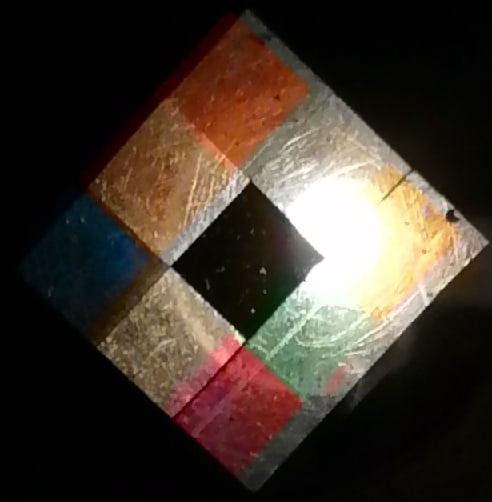
\includegraphics[width=\linewidth]{5}
	\caption{Определение разрешенных направлений поляроида}
	\label{ris 5}
\end{wrapfigure}
Поворачивая поляроид вокруг направления луча, а чёрное зеркало вокруг вертикальной оси, методом последовательных приближений добьемся
наименьшей яркости отражённого пятна. Определим разрешённое направление поляроида. По лимбу оно равно $ x = 45 $. \par
Поставим вместо чёрного зеркала второй поляроид и определим
его разрешённое направление, скрестив поляроиды. Получаем $ x = 15 $. 
\clearpage

\subsection{Определение показателя преломления эбонита}
Поставим на скамью вместо чёрного зеркала (рис. 4) эбонитовую
пластину и определим по лимбу угол Брюстера. Получаем $ \theta =(57 \pm 2) ^\circ$. 

Отсюда получаем, что $ n = \tg \theta \approx 1.53 \pm 0.06 $. Табличное значение показателя преломления эбонита $ n = 1.6 $ -- $ 1.7 $.

\subsection{Исследование стопы}
\begin{wrapfigure}{l}{0.35\linewidth}
	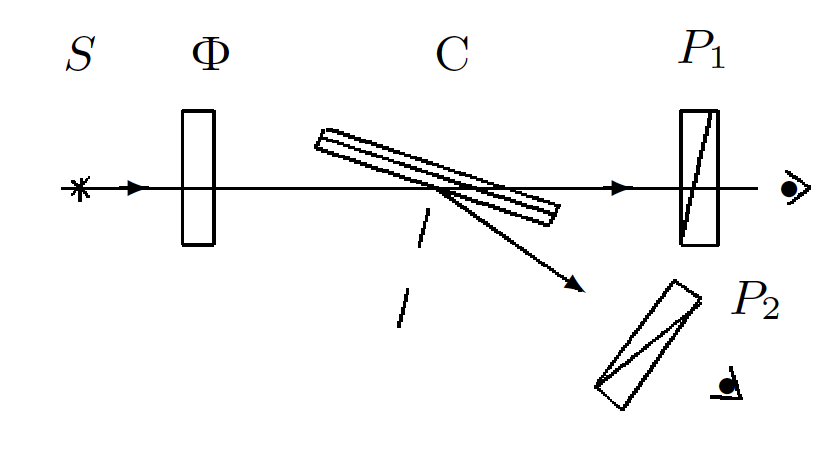
\includegraphics[width=\linewidth]{6}
	\caption{Исследование стопы}
	\label{ris 6}
\end{wrapfigure}
Исследуем характер поляризации света в преломлённом и отражённом от стопы лучах. 
Для этого поставим вместо эбонитового зеркала (рис. 5) стопу стеклянных пластинок под углом Брюстера.
Осветим стопу неполяризованным светом и, рассматривая через поляроиды (рис. 6) отражённый от стопы и преломлённый лучи, определим в них ориентацию вектора $ \mathbf{E} $. Получаем, что в отраженном свете присутствует преимущественно вертикальная линейная поляризация вектора $ \mathbf{E} $, а в преломленном свете преобладает перпендикулярная ей горизонтальная поляризация.

\subsection{Двоякопреломляющие пластины, выделение пластин $ \lambda/2,  \lambda/4 $}
\begin{wrapfigure}{l}{0.35\linewidth}
	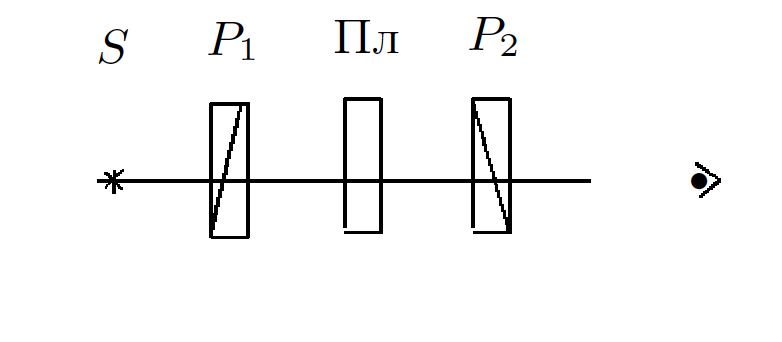
\includegraphics[width=\linewidth]{7}
	\caption{Определение главных направлений в пластинках}
	\label{ris 7}
\end{wrapfigure}
Поставим кристаллическую пластинку
между скрещенными поляроидами $P_1$ и $P_2$. Вращая пластинку вокруг направления луча и наблюдая за интенсивностью света, проходящего сквозь второй поляроид, определим, при каком условии главные направления пластинки
совпадают с разрешёнными направлениями поляроидов. Повторим опыт для второй пластинки.\\
\\
\begin{center}
    Пластина 1 \hspace{1cm} Пластина 2 \\
    $min: 30^{\circ}, 120^{\circ}$ \hspace {1cm} $min: 10^{\circ}, 105^{\circ}$ \\
     $max: 72^{\circ}$ \hspace {1.9cm} $max: 70^{\circ}, 154^{\circ}$
\end{center}
\par Минимумы и максимумы интенсивности чередуются через $45^{\circ}$, главные плоскости пластин совпадают с разрешёнными направлениями поляроидов при максимальной интенсивности.

Добавим к схеме зелёный фильтр; установим разрешённое направление поляроида горизонтально, а главные направления исследуемой пластинки — под углом $45^{\circ}$ к горизонтали. \par 
Пластинка $\lambda/2$ не меняет характер поляризации, при её повороте \textit{меняется интенсивность}, а поляризация остаётся линейной. \par
Пластинка $\lambda/4$ создаёт сдвиг фаз $\pi/2$ между колебаниями - эллиптическая поляризация. Эта пластинка \textit{не меняет интенсивность} при повороте.

\subsection{Быстрая и медленная оси $ \lambda/4 $}
\begin{wrapfigure}{r}{0.35\linewidth}
	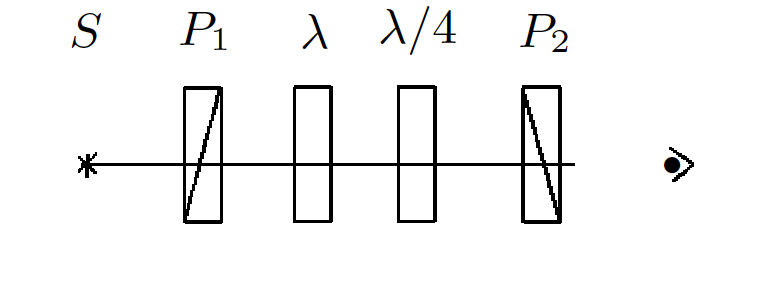
\includegraphics[width=\linewidth]{8}
	\caption{Определение направлений большей и меньшей скорости}
	\label{ris 8}
\end{wrapfigure}
Для определения "<быстрой"> и "<медленной"> оси в пластинке $ \lambda/4 $ оставим между скрещенными поляроидами пластинку чувствительного оттенка, имеющую вид стрелки, и убедимся, что эта пластинка не меняет поляризацию зелёного света. Уберем зелёный фильтр и убедимся, что стрелка имеет пурпурный
цвет. Это объясняется тем, что зелёная компонента линейно поляризованного света при прохождении пластинки не меняет поляризации и задерживается вторым поляроидом.

Добавим к схеме пластинку $ \lambda/4 $ (рис. 7), главные направления которой совпадают с главными направлениями пластины $ \lambda $ и ориентированы
под углом $ 45^\circ $ к разрешённым направлениям скрещенных поляроидов.
При повороте рейтера со стрелкой на $ 180^\circ $ вокруг вертикальной оси
цвет стрелки меняется от зелёно-голубого до оранжево-жёлтого. В первом случае у нас "<быстрая"> ось (они совпадают), во втором --- медленная.

\subsection{Интерференция поляризованных лучей}
\begin{wrapfigure}{r}{0.3\linewidth}
	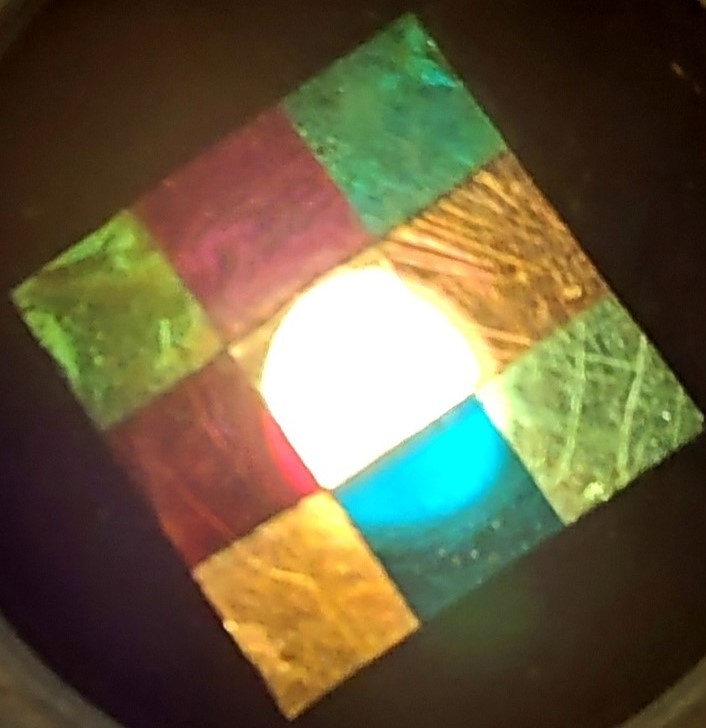
\includegraphics[width=\linewidth]{9}
	\caption{Интерференция поляризованных лучей}
	\label{ris 9}
\end{wrapfigure}
Исследуем интерференцию поляризованных лучей. Для этого расположим между скрещенными поляроидами мозаичную слюдяную пластинку. Она собрана из 4-х узких полосок слюды, лежащих по сторонам квадрата (две полоски "<толщиной"> $ \lambda/4 $ и по одной --- $ \lambda/2 $ и $ 3\lambda/4 $). В центральном квадратике слюды нет. Главные направления всех пластинок ориентированы параллельно сторонам квадрата.

Вращая пластинку, пронаблюдаем за изменениями в отдельном квадратике. У нас изменяется интенсивность. 

Не трогая пластинки, повращаем второй поляроид. Отличие в том, что теперь изменяется (инверсируется) цвет пластинок также с периодичностью  $\pi/4$.

\section{Вывод}
Изучили явления связанные с поляризацией света: определили разрешённые направления поляроидов и с помощью них проводили следующие опыты. Рассмотрели угол Брюстера, с помощью него определили показатель преломления эбонита. Для двоякопреломляющих пластин определили главные направления, а так же тип пластинок --- $\lambda /4$ и $\lambda/2$. Также исследовали пластинку чувствительного оттенка, определили быструю и медленную оси и рассмотрели эффекты, происходящие при прохождении света через комбинацию пластинок. Получили эллиптически поляризованную волну, рассмотрели интерференцию поляризованных лучей в мозаичной слюдяной пластинке.

\end{document}
